% !TeX root = ../../thesis.tex
\chapter{Introduction}\label{ch:introduction}

\instructionsintroduction
\section{Semiconductor Image Sensors}

\section{Towards Ultra-High Resolution Imagers}

\subsection{Replacing Color Filters with Color Splitting Waveguides}
\subsection{Absorption Efficiency vs Response Time: A trade-off}

\begin{itemize}
    \item Increasing the electric field (Single photon avalanche diode)
    \item Reducing the effective charge collection depth
    \item Antireflection, backscattering structures, and deep trench isolation technologies
\end{itemize}

\subsection{Beyond Silicon Detectors}
\begin{itemize}
    \item Provide alternatives for visible light detection (Ge, InGaAs, Organics)
    \item Introduce perovskites as an alternative
    \item Give examples for perovskites integrated with read-out circuits (high-level) (Wenya paper literature review)
\end{itemize}


\section{Perovskite-Based Photodetectors}

\subsection{Properties of Perovskites}

\begin{figure}[htbp]
    \centering
    % First image (top)
    \begin{subfigure}[b]{\textwidth}
    \centering
        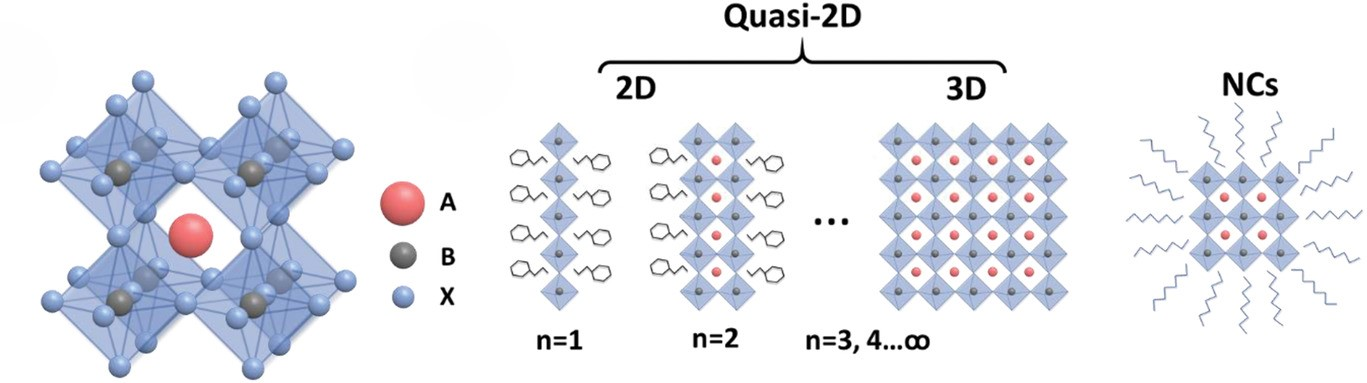
\includegraphics[width=0.85\linewidth]{chapters/introduction/image/perovskite_structure.jpg}
        \caption{}
        \label{fig:ch1:perovskite structure}
    \end{subfigure}

    \vspace{0.5cm}
    
    % Second image (bottom)
    \begin{subfigure}[b]{\textwidth}
    \centering
    %\hspace{-1.4cm}
        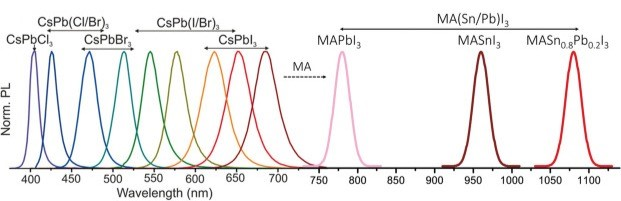
\includegraphics[width=0.85\linewidth]{chapters/introduction/image/bandgap_tunability.jpg}
        \caption{}
        \label{fig:ch1:bandgap_tunability}
    \end{subfigure}
    
    \caption{(a) Reproduced from \cite{Lei2021MetalApplications}. (b) Reproduced from \cite{Gholipour2020BandgapMaterials}.}
    \label{fig:ch1:perovskite_strucutre_bandgap}
\end{figure}



The term perovskite was first used in 1839 to name the newly discovered naturally occurring mineral calcium titanate (\ch{CaTiO_3}), but it took 170 years before perovskites were integrated into photovoltaic devices by the Miyasaka group in 2009 \cite{Kojima2009OrganometalCells}. Since then, intensive scientific research has enabled single-junction perovskite cells to surpass the power conversion efficiency (PCE) of the much more mature single-junction Si solar cells ($> 26\%$). Meanwhile, perovskite-Si tandem solar cells have demonstrated PCEs beyond the Shockley-Queisser limit ($>34\%$), establishing themselves as one of the most dominant candidates for next-generation solar technologies \cite{Hasan2024StabilityReview, Noman2024ATechnology}. This rapid growth of perovskite-based solar cell technology, from its inception to its commercial realization within 15 years, is attributed to both practical advantages and the exceptional optoelectronic properties of perovskites, as well. Practical advantages include, but are not limited to, low-cost production, dependence on abundant materials, and versatile fabrication through a wide variety of methods. On the other hand, some remarkable optoelectronic properties of perovskites are their tunable and direct bandgap, high absorption coefficient, low exciton binding energy, defect tolerance, and long carrier lifetime. 

Perovskites can be divided into three groups, each of which has distinct properties: three-dimensional (3D), two-dimensional (2D) or quasi-2D, and zero-dimensional (0D) perovskites (Fig.~\ref{fig:ch1:perovskite structure}). 3D perovskites can be generally described by the \ch{ABX_3} formula, where A is a 12-fold-coordinated monovalent cation such as methylammonium (\ch{MA^+}), formamidinium (\ch{FA^+}), or cesium (\ch{Cs^+}), B is a 6-fold-coordinated inorganic divalent inorganic cation such as lead (\ch{Pb^{2+}}) and tin (\ch{Sb^{2+}}), while X is a strongly electronegative monovalent halide anion (\ch{I^-}, \ch{Br^-}, and \ch{Cl^-}). As a result, mixed compositions can be pursued for each lattice site, enabling the tuning of the perovskite's bandgap across a wide range of energies (spanning from near ultraviolet (UV) to near infrared (NIR)), depending on the desired application (Fig.~\ref{fig:ch1:bandgap_tunability}).

say about tolerance factor


\subsection{From Solar cells to Photodetectors}

The rapid advancements of perovskite-based solar cells sparked interest for their use in alternative optoelectronic applications, including photodiodes, light-emitting diodes (LEDs), and lasers. While solar cells operate without external bias, photodetectors typically operate in the reverse bias regime (to promote faster carrier extraction), while lasers and LEDs operate in the forward bias regime (to promote radiative charge recombination). While the diode structure is similar for all applications, the different operational regimes introduce distinct challenges for each use. Nevertheless, the operation of solar cells and photodiodes is more closely related, as they both depend on the efficient extraction of the photo-generated carriers. This process relies on the photovoltaic effect, during which the incoming light is absorbed by the active material, as long as its wavelength is equal or smaller than the bandgap, leading to the generation of electron-hole pairs (or excitons). Under the effect of the built-in potential (which may be complimented by an additional field through reverse bias), the charge carriers are extracted and collected at the respective contacts as photocurrent. 

The structure that allows this process is a p-i-n diode, where the perovskite is the intrinsic layer and the built-in potential is defined by a hole transport layer (HTL) and an electron transport layer (ETL), as shown in Fig. xx. Typically, wide-band gap materials are used as transport layers, so as to act as blocking layers for the opposite type of carriers. However, it has to be noted that the diode structure is not the only perovskite-based architecture, alternative include photo conductors, and photo resistors, whose properties are summarized in the Fig. xx. However, in this work the goals is integration on imagers circuits, and fast extraction time, so the photo-diode architecture is the only one considered. 




\begin{itemize}
    \item Schematic for absorption, extraction collection
    \item Solar cell structure, role of transport layer
    \item Transition of photodetectors - use of same structure 
    \item Advantages of photodiodes compared to transistors, conductors, resistors 
    \item Some examples of perovskite-based photodetectors (low dark current - and what affects, fast extraction, X-Ray detection, flexibility, etc)
    \item Figures of merit for photodiodes 
\end{itemize}

\subsection{Scalable, High-Temperature Perovskites}

The vast majority of studies on perovskite-base optoelectronic devices rely on the use of solution processed methods, and specifically spin-coating. This is not surprising, considering that spin-coating is a technique that is simple, easily accessible, and has low cost. These characteristics make it highly suitable for rapid prototyping and exploration of various material combination that can promote efficiency or stability. For example, during solution preparation it is common to include various additives that in turn can help modulate morphology, optimize energy level-alignment or eliminate hysteresis \cite{Liu2020ACells}. However, cell fabrication through spin-coating is not transferable to industry, due to limitation is throughput and large-area deposition. For example, a commonly used technique, anti-solvent processing has been shown to be challenging to scale-up\cite{Saki2021Solution-processedCells}.

Significant efforts have been made to explore alternative fabrication techniques that enable the scalable deposition of perovskite-based devices. Such methods involve solution-processed approaches (such as inkjet printing and spray coating) or vacuum-processed on (such as chemical vapor deposition or thermal evaporation). Among those, thermal evaporation is the most mature one, and in 2020 it enabled the fabrication of 21 $cm^2$ mini modules with the superior efficiency of 18.13\% \cite{Vaynzof2020TheProcessing, Li2020HighlyMini-modules}. Besides scalability, thermal evaporation offers the advantage of not necessarily requiring a post-deposition thermal annealing step, rendering highly attractive for applications that require the use of flexible substrates \cite{Becker2019LowExperimentation}. Besides that, it avoids the use of toxic solvents, allows for precise control of the deposited thickness, and prevents the risk of damaging the underlying layers in tandem structures \cite{Zhang2020TowardCells, Forgacs2017EfficientCells}

Despite the advantages of using thermal evaporation for the deposition of perovskite-based optoelectronic devices, several limitations still exist. For instance, the high vacuum pressure and low sticking coefficient of \ch{MA^+} renders its evaporation rather complicated \cite{Kim2020DepositionCH3NH3PbI3Perovskite}. At the same time, the inclusion of additives, which is crucial for improving the performance/stability of solution-processed films, is not compatible with evaporation. Lastly, evaporated perovskite films tend to have significantly smaller grain sizes, which may compromise their stability against moisture or limit device performance due to their higher defect density \cite{Vaynzof2020TheProcessing, Wang2017Scaling}.


Besides the use of spin-coating as the fabrication technique, research around perovskite optoelectronic devices is mainly focused on the use of hybrid organic-inorganic perovskites, where the A-site cation is a mixture of \ch{MA^+}, \ch{FA^+}, and/or \ch{Cs^+}, leading to optimal performances \cite{Zhang2021All-inorganicCells}. However, perovskites that contain organic molecules are more sensitive to thermal degradation. For instance, it was shown that methylammonium-based perovskites decompose into methylamine, hydrogen iodide, and lead iodide for temperatures beyond 100 \degree C. This limitation sets hybrid organic-inorganic perovskites unsuitable for applications with high thermal budget, which may be imposed by intrinsic (triggering of self-heating mechanisms through resistive loses) or extrinsic factors (high ambient temperature, high temperature post processing) \cite{Handa2019LargePerovskite, Dong2021SupportingFilm, Li2022StructureTemperatures}. Such a condition is imposed in the case of color-splitting waveguides, which have to be bonded to the underlying photodetector structure at temperatures beyond 250 \degree C. 

Under these circumstances, all-inorganic perovskites, in the \ch{CsPbI_{x}Br_{3-x}} for $1 \le x \le 3 $ family become and attractive solution. 

\textbf{Advantages of all-inorganic perovskites: }

\begin{itemize}
    \item $CsPbI_3$ exists in several phases:
    \item The cubic $\alpha$-phase
    \item Two quasi-perovskite phases: The tetragonal $\beta$-phase, and the orthorhombic $\gamma$-phase
    \item The non-perovskite, orthorhombic, yellow $\delta$-phase \cite{Steele2019ThermalFilms,Mali2021ImplementingCells}. 
       
    
    \item The $\alpha-$, $\beta-$, and $\gamma-$phases are similar in structure in properties
    \item As a result, they are commonly referred to as the "black phase" without proper distinction between them \cite{Steele2019ThermalFilms, Yan2020DeterminationFilms, Sutton2018CubicExperiment}

    \item The naming as black and yellow phase comes from the color films, which indicates their bandgap (xx for black phase, xx for yellow phase)

    \item Therefore only the black phases are interesting for optoelectronic applications \cite{Burwig2018CrystalFilms, Steele2022AnFilms}.

    \item The black phases of $CsPbI_3$ are stable at high temperature (> what number)

    \item It is possible to kinetically trap the black phase at room temperature through rapid cooling

    \item However, the yellow phase emerges almost instantaneously upon exposure to ambient moisture \cite{Steele2019ThermalFilms}.

    \item What is triggering the conversion? Give some energy transition diagrams (Refer to Gibbs free energy and tolerance factor)

    \item Besides encapsulation, many strategies have been proposed to increase the stability of $CsPbI_3$ in ambient conditions, namely: introduction of stabilizing agents, passivation of surfaces, stress introduction through laser writing, and doping with other materials (replacing iodine with other halides or replacing lead with Bismuth and tin). \cite{Li2018SurfaceCells, Li2020ApproachesCells, Steele2022AnFilms, MinSim2018PhaseApplications} - check more citations  
    
\end{itemize}

\subsection{State of the art for evaporated, all-inorganic perovskites}

Besides the use of inorganic, vacuum-deposited perovskites, the whole stack has to be inorganic and vacuum deposited. This is a condition that has not been explored so far, except for limited occasions. 

\textbf{Good discussion and references for Metal Oxides as trasnport layers happens here \cite{Yang2023InvertedPassivation}}.


\section{Scope and Aim of This Thesis}

It is common to see solution-processed layers in combination with thermally evaporated perovskites. \textit{This goes in stark contrast to the solvent-free nature of thermal evaporation}. It is important to develop truly all-inorganic and all-evaporated perovskite-based photodetectors. 



\begin{itemize}
    \item Develop an all-inorganic perovskite diode (many reports use inorganic perovskites with organic TLs - this defies the purpose of using an inroganic absorber)
    \item Evaluate the deposition conditions on performance and repeatability of the photodetector
\end{itemize}


%%%%%%%%%%%%%%%%%%%%%%%%%%%%%%%%%%%%%%%%%%%%%%%%%%
% Keep the following \cleardoublepage at the end of this file, 
% otherwise \includeonly includes empty pages.
\cleardoublepage

% vim: tw=70 nocindent expandtab foldmethod=marker foldmarker={{{}{,}{}}}
